\documentclass[%
 reprint,
superscriptaddress,
%groupedaddress,
%unsortedaddress,
%runinaddress,
%frontmatterverbose, 
%preprint,
%showpacs,preprintnumbers,
nofootinbib,
%nobibnotes,
%bibnotes,
 amsmath,amssymb,
 aps,
%pra,
%prb,
%rmp,
%prstab,
%prstper,
%floatfix,
colorlinks = true, 
linkcolor = blue, 
urlcolor = blue, 
citecolor = blue, 
anchorcolor = blue,
]{revtex4-2}

\usepackage{graphicx}% Include figure files
\usepackage{dcolumn}% Align table columns on decimal point
\usepackage{bm}% bold math
\usepackage{lipsum}
\usepackage{amsmath,amssymb}
\usepackage{dsfont}
\usepackage{float}
\usepackage{array}
\makeatletter
\let\newfloat\newfloat@ltx
\makeatother
\usepackage{algorithm}
\usepackage{algpseudocode}
\usepackage{multirow}
\usepackage{colortbl}
\usepackage{booktabs}
\usepackage{stmaryrd}
\usepackage{comment}
% \usepackage{hyperref}
\usepackage{tcolorbox} % For fancy boxes
\usepackage{color}
\usepackage{todonotes}
\usepackage{amsthm}
\usepackage{hyperref}
\usepackage{physics}

\usepackage{showyourwork}



\newcolumntype{C}{>{$}c<{$}}

\AtBeginDocument{%
  \heavyrulewidth=.08em
  \lightrulewidth=.05em
  \cmidrulewidth=.03em
  \belowrulesep=.65ex
  \belowbottomsep=0pt
  \aboverulesep=.4ex
  \abovetopsep=0pt
  \cmidrulesep=\doublerulesep
  \cmidrulekern=.5em
  \defaultaddspace=.5em
}

\usepackage{verbatim}
\usepackage[left=2cm, right=2cm, top=2cm]{geometry}

\usepackage[normalem]{ulem}
\usepackage[utf8]{inputenc}
\usepackage{epigraph}
\usepackage{siunitx}
\usepackage[english]{babel}
\usepackage{listings}
\usepackage{graphicx}
\usepackage[utf8]{inputenc}
\usepackage{listings}
\usepackage{matlab-prettifier}
\usepackage{xcolor}
\usepackage{amsfonts}
\usepackage{amsmath}
\usepackage{amssymb}
\usepackage{amsthm}
%\usepackage[showframe]{geometry}
\newcolumntype{P}[1]{>{\centering\arraybackslash}p{#1}}
\newcolumntype{M}[1]{>{\centering\arraybackslash}m{#1}}
\usepackage{braket}
\usepackage{xcolor}
\usepackage[colorlinks = true,
            linkcolor = blue,
            urlcolor  = blue,
            citecolor = blue,
            anchorcolor = blue]{hyperref}


\newcommand{\MYhref}[3][blue]{\href{#2}{\color{#1}{#3}}}%



\newtheorem{postulate}{Postulate}
\newtheorem{lemma}{Lemma}
\newtheorem{theorem}[lemma]{Theorem}
\newtheorem{corollary}[lemma]{Corollary}
\newtheorem{prop}[lemma]{Proposition}
\newtheorem{definition}[lemma]{Definition}
\newtheorem{remark}[lemma]{Remark}
\newtheorem{example}[lemma]{Example}

\newcommand{\tit}{\tilde{t}}

\newcommand{\eps}{\epsilon}
\newcommand{\Eps}{\dot{\mathcal{E}}}
\newcommand{\hN}{\hat{N}}
\newcommand{\hn}{\hat{n}}
\newcommand{\hw}{\hat{w}}
\newcommand{\hh}{\hat{h}}
\newcommand{\hH}{\hat{H}}
\newcommand{\hD}{\hat{D}}
\newcommand{\hK}{\hat{K}}



\newcommand{\be}{\begin{equation}}
\newcommand{\ee}{\end{equation}}

\newcommand{\diff}[2]  {\frac{d #1}{d #2}}

\newcommand{\ob}[1]{\textcolor{blue}{\bf [[[Ollie: #1]]]}}
\newcommand{\ls}[1]{\textcolor{purple}{[Lorenzo: #1]}}
\newcommand{\qb}[1]{\textcolor{purple}{[Quentin: #1]}}
\newcommand{\avi}[1]{\textcolor{red}{[Avi: #1]}}

\newcommand{\package}{\texttt{PyWavelet}}



\begin{document}

\preprint{APS/123-QED}

% \title{Pywavelet: a python-based library for data analysis in the wavelet domain}
% \title{PyWTF: A Python-based code for time-frequency based gravitational wave data analysis library}
% \title{A Python-based code for Time-frequeNcy Transforms (TNT) to be used for gravitational wave data analysis}
\title{Accelerated Python-based codes for Time-frequeNcy Transforms (TNT) for use within gravitational wave astronomy}
% \title{Pywavelet: a python-based library for data analysis in the wavelet domain}


\author{Quentin Baghi}
\affiliation{Paris}
\author{Ollie Burke}
\affiliation{School of Physics and Astronomy, University of Glasgow, University Avenue, Glasgow, G12 8QQ, UK}
\affiliation{Laboratoire des 2 Infinis - Toulouse (L2IT-IN2P3), Université de Toulouse, CNRS, UPS, F-31062 Toulouse Cedex 9, France}
\author{Giorgio Mentasti}
\affiliation{Department of Physics, Imperial College London, Prince Consort Road, SW7 2AZ, London, United Kingdom}
\author{Lorenzo Speri}
\author{Avi Vajpeyi}
\affiliation{Department of Statistics, University of Auckland, 38 Princes St, Auckland, New Zealand}



\affiliation{Fill in}

\begin{abstract}
    Here we present \package, a python-based GPU/CPU agnostic code to compute rapid and accurate time-frequency transforms in the Wilson-Daubechiers-Meyer (WDM) domain. Our implementations are based off JAX and CUDA, with analysis length data streams (millions) of data points being transformed in fractions milliseconds to excellent levels of precision. We give a theoretical discussion on the WDM domain and honest remarks on practical limitations that should be considered when working in the time-frequency domain. We conclude by discussing some of the challenges that will be encountered and could be mitigated via incorporating time-frequency data analyses into future space-based gravitaitonal wave interferometers.
    
    % Scientific exploitation of gravitational wave observations relies on analysis of the complex data and rapid computation of gravitational waveform models. In this work, we present a python-based library for the analysis of gravitational wave data in the time-frequency domain. We describe the implementation of the data analysis tools in this domain and estimate their computational cost. 
    % \ls{place holder}
\end{abstract}

\maketitle
% \tableofcontents

\section{TODOs}

\begin{itemize}
    \item Clarify pixel independence - Explain when/why wavelet coefficients are uncorrelated and limitations (QB has some stuff on this) 
    \item Clarify that this is technically a ``wavelet wavepacket transform" – and what the difference between this and a wavelet transform (Avi can do this) 
    \item Clarify the special treatment in the Nyquist+DC bins (QB + giorgio?).
    \item Prove Equations (19) and (21) in Appendix. 
    \item Direct FFT comparison - Runtime and memory usage vs standard frequency domain analysis
\end{itemize}







\section{Introduction (Literature review, Avi + Lorenzo)}
\ls{What has been done so far:}
Time-frequency analysis is widely used in gravitational-wave astronomy. 
It allows for template-free modeling of source signals~\cite{krolak_1996,Virtuoso2024},  instrumental transients~\cite{robinet2020}, or the simultaneous analysis of both astrophysical signals and terrestrial disturbances~\cite{Cornish_2015}.
Furthermore, time-frequency representations facilitate compact waveform descriptions and robust modeling of non-stationary detector noise. 
Among the various time-frequency techniques, wavelet transforms are exceptionally well-suited for gravitational-wave data analysis due to their inherent ability to provide mathematical basis functions that effectively describe transient and chirping signals.
In certain conditions, these wavelet bases can be constructed to be orthonormal, thereby allowing for exact and reversible transformations between the wavelet and time or frequency domains. 




This paper specifically focuses on the applications of the discrete Wilson-Daubechiers-Meyer (WDM) filter based time-frequency domain in gravitational-wave astronomy, detailing its forward and backward transformations, and introducing an associated Python package designed to streamline its practical implementation.

\ls{What is new here}


\avi{Compare against FFT}
Unlike the Fourier transform, which represents signals using a sum of infinite-duration sine and cosine waves, the wavelet transform uses short, finite-length functions called wavelets. 
This allows wavelets to be localized in both time and frequency -- effective for analyzing non-stationary signals where frequency content changes over time.  
Fourier's infinite-duration basis functions smear temporal information, making it hard to detect transient events. In contrast, wavelets are compactly supported, enabling them to capture localized, time-varying features.


\avi{What is the mother wavelet}
Wavelets are generated from a single ``mother'' wavelet through scaling and shifting, forming a family of ``daughter'' wavelets. 
Each is associated with a coefficient that quantifies its contribution at a specific time and scale. 
The transform is reversible -- the original signal can be reconstructed by summing the weighted wavelets.




\subsection{Conventions (All)}
% Here we need to be clear on our conventions -- suggestions
% \begin{itemize}
% \item Define conventions for fourier transform
% \item bold face roman letters indicate vectors and matrices
% \item bold face greek letters indicate parameter sets
% \item etc. 
% \end{itemize}

We are given a data stream in time domain, consisting of a set of N samples of a \textbf{real} quantity $x$ at times $\{t_k\}_{k=0\dots N-1}$ in a total time of observation $T$
\begin{align}\label{st_definition}
x[k]=x(t_k)\qquad,\qquad k=\{0\dots N-1\}\;,
\end{align}
sampled uniformly with sampling interval $\Delta t = t_{k+1} - t_{k}$ with $T = N\Delta t$. All of the information we have lies in these N points. We define the time sampling rate and the Nyquist frequency as
\begin{align}
r_s&\equiv\frac{1}{\Delta t}\equiv\frac{N}{T}\;,\nonumber\\
f_{\rm max}&=\frac 1 2r_s\;,\nonumber\\
\Delta f &\equiv 1/(2\Delta t)
\end{align}
With that respect, if we set $t_0=0$, we can write $t_k=k\Delta t$. 
% ===========================================================================
% CONTINUOUS NOTATION REMOVED (UNUSED IN THE REST OF THE PAPER)
% ===========================================================================
% The relation between the continuous time and frequency domain is given by:
% \begin{align}
%     x(t) &= \mathcal{F}^{-1}\qty[\tilde h(f) ](t) = \int_{-\infty} ^{+\infty} \tilde h(f) e^{i 2 \pi f t} \dd f ,\\
%     \tilde{x}(f) &= \mathcal{F}\qty[\tilde h(t) ](f) =\int_{-\infty} ^{+\infty} h(t) e^{-i 2 \pi f t} \dd t \, ,
% \end{align}
% \ls{Update the above formula with discrete notation }

In the frequency domain, the data stream $\{x_k\}$ can be discrete-Fourier-transformed to a set of other $N$ complex numbers as
%
\begin{equation}
\label{eq:dft-definition}
%X[p] = \sum_{n = -N/2}^{N/2 - 1}x[n]\exp(\frac{-2\pi i}{N} p n)
X[p] = \sum_{k = 0}^{N-1} x[k]e^{-2\pi i p k/N} % Introduce the definition that we actually use!
\end{equation}
%
for Fourier frequencies $f_{l} = \{-N\Delta f/2, \ldots, -\Delta f, 0, \Delta f, (N/2 - 1)\Delta f\}$. This is convenient since the zeroth frequency bin has been shifted into the middle of the spectrum.

\textcolor{blue}{[Giorgio: I think we have to pick up only one of the two Fourier transforms (i.e. the symmetric or the asymmetric DFT) to avoid confusion. In particular, I'd say we only write and use the one in the code - so maybe we wait to migrate to JAX?]}


\ls{General introduction and motivation for time frequency:}




%--------------------------------------------
% \section{Domains for Gravitational wave data analysis}

%%%%%%%%%%%%%%%%%%%%%%%%%%%%
% \subsection{Gravitational wave data analysis}
\subsection{Time and Frequency Domains (Ollie + Quentin)}
% ===========================================================================
% PLAN
% ===========================================================================
% \begin{itemize}
% \item Discuss matrix formalism in time-domain. Demonstrate simple transformation between time to frequency domains
% \item State useful quantities, likelihood, SNR etc. Derive the Whittle likelihood. Discuss the speed of Whittle in comparison to dense (circulant) time-domain. Can just refer to mine and Sylvain's work on the gaps for this. 
% \item Discuss advantageous and disadvantageous of time-domain GW data analysis. Useful for gaps + ringdown analyses or simply conceptual studies. 
% \end{itemize}


We assume that the output of a gravitational wave detector, $x(t)$, is expressed as a linear combination of a signal, $h(t| \vec{\mu})$, determined by a finite set of (unknown) parameters, $\vec{\mu}$, and instrumental noise, $n(t)$. If we ignore the presence of calibration errors~\cite{Savalle_2022}, the content of a single data stream, i.e., one output channel from one detector, can be written in the time and frequency domain as:
\begin{align}
{x}[k] & = h[k|\vec{\mu}]+ n[t],\\
X[l]& = \tilde{h}[l|\vec{\mu}]+ \tilde{n}[l]
\end{align}
%
where the tilde indicates the Fourier transform. 

In a gravitational wave context it is usual to further assume that the instrumental noise follows a Gaussian distribution characterized by a one-sided PSD, $S_n(f)$, defined such that
\begin{equation}\label{eq:psd_definition}
 \langle \tilde{n}^*[l] \tilde{n}[l'] \rangle = \frac{1}{2} P[l] \delta_{ll'},
\end{equation}
%
where the expectation value $\langle \, \rangle$ is taken over the data generating process. The delta function in the previous equation implies that different frequencies are not correlated.

In reality the noise model is not known perfectly and could vary from the assumption above in a number of ways. For example, the PSD might have a different shape from the reference one \cite{babak2021lisa}, the probability distribution of the noise might not be Gaussian, or the noise might not be stationary, leading to correlations between frequencies. 

% In this work we will continue to assume that the noise is Gaussian and stationary, but we will allow the power spectral density to vary using a parametrized spectral density, $S_n(f) \rightarrow S_n(f|\vec\lambda)$, described by parameters $\vec\lambda$. Then the log-likelihood depends on both sets of parameters, $\vec\mu$ and $\vec\lambda$, and can be written as:
% \begin{align}
%    l &= \ln p(\tilde{x}|\vec\mu,\vec\lambda) \\
%    &= - \ln\bigg{[}2 \pi \frac{1}{4} \det [S_n(f|\vec\lambda)\delta(f-f')] \bigg{]} \\ & - \frac{1}{2} \qty(4 \int_{0}^{\infty} \frac{|\tilde{x}(f) -\tilde{h}(f|\vec{\mu})|^2}{S_n(f|\vec\lambda)} \dd f )
%    % = - \int \ln\left[2 \pi \frac{S_n(f|\vec\lambda)}{4 \Delta f} \right] -\\ \frac{1}{2} \sum_{k = 1}^{n} \frac{|\tilde{x}(f_k) -  \tilde{h}(f_k|\vec\mu) |^2}{\frac{1}{4\Delta f} S_n(f_k|\vec\lambda)}
% \end{align}

% ===========================================================================
% THE LIKELIHOOD PART IS REMOVED BECAUSE UNUSED IN THE REMAINDER OF THE PAPER
% ===========================================================================
% \ls{Remove likelihood and below}
% The first term does not include the $1/2$ factor because the real and imaginary parts of $\tilde{n}(f_k)$ are independent random variables. This follows from the fact that, for a real time series, $\tilde{n}^*(f) = \tilde{n}(-f)$, which combined with Eq.~(\ref{eq:psd_definition}) means that $\langle \tilde{n}(f) \tilde{n}(f') \rangle = 0$ for $f$, $f'>0$. 
% This allows equation~\ref{eq:psd_definition} to be rewritten as
% \begin{equation}
% \langle \Re[\tilde{n}(f)]^2\rangle = \langle \Im[\tilde{n}(f)]^2\rangle = \frac{\langle | \tilde{n}(f)|^2\rangle}{2}= \frac{S_n(f| \vec\lambda)}{4}\delta(0) \, .
% \end{equation}

% We can define the inner product as
% \begin{equation}
%     \braket{a}{b} = 2 \Re \int_{-\infty}^{\infty} \frac{\tilde{a}^* (f) \tilde{b}(f)}{S_n(f)} \dd f \, .
% \end{equation}

% \textcolor{blue}{[Giorgio: how about rewriting the frequency domain analogy in the discrete case to have consistency with the discrete wavelet?]}


% The representation of the data in the time-frequency can be obtained starting from the following expressions:




%------------------------------------
% \subsection{Data analysis in the time-frequency domain}
\subsection{The Time-Frequency domain (Lorenzo + Giorgio)}
\begin{itemize}
\item This section should really focus on the conventional short fourier transform (SFT). Lorenzo, you have experience with this and I think you should focus on this section. 
\item I want to understand why choose the WDM domain over the SFT domain.  
\item I'm sure matrix formalism can be tied to this as well. Easily.
\item Discuss PSD, derive the form suitable for time-frequency.
\end{itemize}

\section{The Wilson-Daubechiers-Meyer (WDM) transform (Lorenzo + Giorgio + Quentin)}
\begin{itemize}
\item Now discuss the WDM domain. There is already a lot of content here. 
\item Matrix formalism, relating time and frequency domains straight to time-frequency. 
\item Discuss backward and forward transformations in detail. Show that one is the inverse of the other (should be easy in matrix formalism). 
\item Discussion of inner product (point-wise multiplication), likelihood and noise generation. 
\item Derivation of the PSD. 
\end{itemize}

The wavelet domain considers a transformation of \eqref{st_definition} that takes the original N points and reshape them into a $N_t\times N_f$ grid, where then
\begin{align}\label{NtNf_def}
N=N_t\,N_f\;,
\end{align}
must hold. The underlying idea, is to chunk the data stream into $N_t$ chunks and to perform a frequency analysis of each one of those. Please note that N is fixed, but $N_t$ is an arbitrary choice you can make. The only constraint is obviously $1\le N_t\le N$. Consequently, the constraint applies for $N_f$: $1\le N_f\le N$.
Given that choice we can define the spacing in both time and frequency with respect to the grid with area $N = N_{t}N_{f}$
\begin{align}\label{DTDF}
\Delta T&\equiv\frac{T_{\text{obs}}}{N_t}\; \qquad \text{grid time spacing},\nonumber\\
\Delta F&\equiv\frac{f_{\rm max}}{N_f} \qquad \text{grid frequency spacing}\,.
\end{align}
One immediately sees that,
\begin{align}
\Delta T &= \frac{T_{\text{obs}}}{N_{t}} = \frac{N\Delta t}{N_{t}} = \frac{N_{t}N_{f}\Delta t}{N_{t}} = N_{f}\Delta t \\
\Delta F &= \frac{f_{\text{max}}}{N_{f}} = \frac{1}{2N_{f}\Delta t} = \frac{1}{2\Delta T}
\end{align}
This final expression shows how the Nyquist theorem still holds. Once you fix $N_t$ (or equivalently $N_f$, $\Delta T$ or $\Delta F$) the grid is uniquely identified.

% ===========================================================================
% PART REMOVED BECAUSE TOO LONG
% ===========================================================================
% \textcolor{blue}{[Giorgio: I would make this part shorter or move it to some appendix even if it is instructive it is space consuming] We can stop here and understand what happens in various limiting cases. Given that $N = N_{t}N_{f}$, by specifying the number of frequency slices this will determine the number of time slices. Through calculation, we determine that 
% \begin{equation}
% \Delta T = 
% \begin{cases} 
% T_{\text{obs}} & \text{if } N_{f} = N \Rightarrow N_{t} = 1\,, \ \text{full frequency resolution}, \\
% \Delta t & \text{if } N_{f} = 1 \Rightarrow N_{t} = N\,, \ \text{full time resolution}.
% \end{cases}
% \end{equation}
% The first case shows that if $N_{f} = N$ then the spacing in time is the entire observation. In other words, we have a single time-bin and thus there would be zero time resolution (only frequency resolution). Similarly, if $N_{f} = 1$, we learn that the spacing in time is given by the original time-series (zero frequency resolution, only time resolution). A similar argument for $\Delta F$ can be understood
% \begin{equation}
% \Delta F = 
% \begin{cases} 
% \frac{1}{2T_{\text{obs}}} & \text{if } N_{f} = N \Rightarrow N_{t} = 1\,, \ \text{full frequency resolution}, \\
% f_{\text{max}} & \text{if } N_{f} = 1 \Rightarrow N_{t} = N\,, \ \text{full time resolution}.
% \end{cases}
% \end{equation}
% Notice that we find $\Delta F = \Delta f / 2$. This is not problematic, and simply a matter of convention. Understand that Each cell will have constant area, given by $\Delta F \Delta T = 1/2$. From a signal processing perspective, the wavelet domain can be thought of as a mix between the time and frequency domain -- possessing advantages and disadvantages of both.}

\subsection{Forward transform}

For a given time series $x[k]$, the WDM transform represents the data through the coefficients %can be rewritten in the form aligned with the notation in eqs.8-9 of \footnote{\url{https://docs.scipy.org/doc/scipy/tutorial/signal.html\#equation-eq-stft-windowing}}.
\begin{align}
\label{wnm_def}
w_{nm}=\sum_{k=0}^{N-1}x[k]g_{nm}[k]\;,
\end{align}
where $n$ corresponds to the time index and $m$ corresponds to the frequency (or scale) index. The functions $g_{nm}[k]$ are the WDM basis elements, which are chosen to be (quasi-)orthonormal:
\begin{align}
\label{eq:orthonormality}
\sum_{k=0}^{N-1}g_{nm}[k]g_{pq}[k]=\delta_{np}\delta_{mq}\;,
\end{align}
The basis elements are defined in closed form in the frequency domain, as
\begin{align}
\label{eq:gnm}
\tilde g_{mn}(f) & = e^{-2 i \pi f n \Delta T}\left( C_{nm}\tilde\phi(2 \pi f -m\Delta\Omega) \right. \nonumber \\
& \left. +C^*_{nm}\tilde\phi(2\pi f+m\Delta\Omega)\right)
\end{align}
where $\phi$ is the Meyer window, defined in the frequency domain by
\begin{align}
\tilde\phi(\omega) &= \begin{cases}
\frac{1}{\sqrt{\Delta \Omega}} & |\omega|<A \\
\frac{1}{\sqrt{\Delta \Omega}} \cos \left[\frac{\pi}{2}\,\nu_d\left( \frac{|\omega|-A}{B}\right)\right] & A \leq|\omega| \leq A+B \\
0 & \text{otherwise.}
\end{cases}
\end{align}
where $\omega = 2 \pi f$ are angular frequencies, which are discretized as
\begin{equation}
    % \omega_l = \frac{2\pi l}{2\Delta t}\frac{2}{N}
    \omega_l = \frac{2\pi l}{N \Delta t}
\end{equation}
and $\nu_d(x)$ is the normalized incomplete Beta function
\begin{align}
\nu_d(x)=\frac{\int_0^x y^{d-1}(1-y)^{d-1} d y}{\int_0^1 y^{d-1}(1-y)^{d-1} d y}\;.
\end{align}
By construction, $\tilde\phi$ has a limited frequency bandwidth which is controlled by the parameter $A$. The smoothness of the window (how it drops from one to zero) is controlled by the parameter $d$. The parameter $\Delta \Omega$ depends on the frequency resolution
\begin{equation}
    \Delta\Omega = 2 \pi \Delta \tilde{F},
\end{equation}
where $\Delta \tilde{F} = \Delta F \Delta t$ is the normalized frequency resolution.
The parameter $B$ depends on $\Delta\Omega$ and $A$ as
\begin{equation}
    B = \Delta\Omega - 2A
\end{equation}
In our implementation, we set $A =\Delta\Omega/4$ and therefore $B = \Delta\Omega/2$. This means that the window is non-zero when $|\omega| \leq 3 \Delta\Omega/4$.

By using the definition of WDM transform in Eq.~\eqref{wnm_def} and the basis functions in Eq.~\eqref{eq:gnm}, one can show that
\begin{align}
w_{n m} &= \sqrt{2}(-1)^{nm}\, \Re\,\Delta t\, C_{n m}\, x_m[n]
\end{align}
The coefficient $C_{nm}$ is alternatively real and complex depending on the value of $n + m$, and can be expressed analytically as
\begin{align}
C_{nm}=e^{\frac{i\pi}{4}(1-(-1)^{n+m})}
\end{align}% eq:dft-definition
The quantity $x_m$ is as a discrete convolution of the data DFT with a shifted window in the frequency domain:
\begin{align}
x_m[n] = \sum_{l=-N_t / 2}^{N_t / 2-1}  e^{-2 \pi i l n / N_t} \,X\left[l+ m N_t/2\right] \tilde\phi[l],
\end{align}
where $X[p]$ is the input data DFT defined in Eq.~\eqref{eq:dft-definition}.


%

\subsection{Backward transform}

The original data stream is recovered by applying the backward WDM transform to the coefficients:
\begin{align}
\label{eq:inverse_wavelet_decomposition}
x[k]=\sum_{n=0}^{N_t-1}\sum_{m=0}^{N_f-1}w_{nm}g_{nm}[k]\;,
\end{align}
where $g_{nm}[k]$ are the wavelet basis elements and $\omega_{nm}$ coefficients of those basis elements.

% \textcolor{blue}{[Giorgio: I would make this part shorter or move it to some appendix even if it is instructive it is space consuming] Notice here that in the limit as $N_{f}\rightarrow N$ the series above \eqref{eq:inverse_wavelet_decomposition} approaches as Fourier series. To be concrete, if $N_{f} \rightarrow N$, then $N_{t}\rightarrow 1$ since $N = N_{t}N_{f}$ and, from the definition of the (inverse) discrete fourier transform, observe that 
% \begin{align}
% h(t_{k}) &= \frac{1}{N}\sum_{m = 0}^{N -1}\tilde{h}(f_{m})e^{2\pi i f_{m}t_{k}} = \sum_{m = 0}^{N - 1}\omega_{0m}g_{0m}[k]\, ,\nonumber
% \end{align}
% with a factor $1/N$ absorbed into the basis coefficients $\omega_{0m}$. Hence, for the Fourier series, we identify $g_{0m}[k] = \exp(2\pi i f_{m}t_{k})$ as the Fourier basis elements and $\omega_{0m} = \tilde{h}(f_{m})$ as the Fourier coefficients.}
% \textcolor{blue}{[Giorgio: we didn't show it actually, do we rather reference something?]} 


\section{\package\ Package}

\label{sec:code_package}

The \package\ package provides implementations of the Wilson–Daubechies–Meyer (WDM) transform for gravitational-wave data analysis. It includes two main backends:

\begin{enumerate}
    \item \textbf{NumPy implementation}: a implementation based on the reference code at \url{https://github.com/XGI-MSU/WDMWaveletTransforms}. This version runs entirely on the CPU.
    \item \textbf{Vectorized JAX and CuPy implementations}: these versions are vectorized to exploit JAX's and CuPy's GPU-accelerated array operations to deliver orders-of-magnitude speedup on suitable hardware. 
\end{enumerate}

In the remainder of this section, all timing results obtained via the NumPy backend were recorded on the CPU, whereas all results for the JAX and CuPy backends were recorded on the GPU (note that while we only show the JAX timings on the GPU, the JAX implementation is CPU/GPU agnostic). 
All the results are obtained using 64-bit floating point precision, and the first evaluation of each analysis is discarded (for any just-in-time compilation to be executed).
Additionally, in order to make the results reproducible, they have been produced on \textbf{Google Colab}, using the T4 GPU runtime. 
The hardware specifications for the machine are:

\begin{itemize}
    \item \textbf{GPU:} 1× Tesla K80 (compute capability 3.7, 2496 CUDA cores, 12 GB GDDR5 VRAM)
    \item \textbf{CPU:} 1× single‐core hyper‐threaded Intel Xeon Processor @ 2.3 GHz (1 core, 2 threads)
    \item \textbf{RAM:} approximately 12 GB
\end{itemize}

\subsection{Performance: Runtime Scaling}
\label{subsec:runtime_scaling}

Figure~\ref{fig:runtime_forward} shows the runtime $N$ (in seconds) of the forward WDM transform (frequency domain to WDM domain) for a monochromatic test signal as a function of data length. The three curves correspond to the CuPy (gray), NumPy (red) and JAX (teal) implementations. \avi{TODO: plot again with N on x axis}.

\begin{figure}[h]
    \centering
    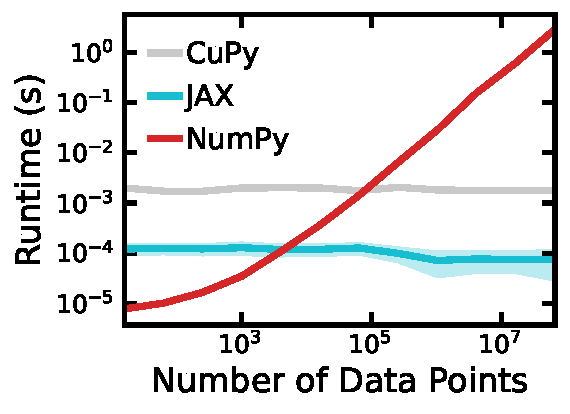
\includegraphics[width=1\linewidth]{figures/runtimes.pdf}
    \caption{\textbf{Runtime of the forward WDM transform versus data length}. The data are monochromatic signals of different length $N$ transformed from frequency domain to WDM domain. CuPy (gray) and JAX (teal) remain nearly constant in runtime due to vectorization on the GPU, whereas NumPy (red) exhibits an increasing runtime for larger $N$. Note that for small $N\lesssim 2^{20}$, the NumPy version is faster; beyond $N\approx 2^{20}$, the vectorized JAX and CuPy implementations outperform NumPy. Code to reproduce this plots can be found here:\url{pywavelet.github.io/pywavelet/examples/runtime.html}.}
    \label{fig:runtime_forward}
\end{figure}


As visible in Figure~\ref{fig:runtime_forward}, the NumPy implementation’s runtime grows approximately linearly with $N$, since each operation is performed in sequence on the CPU. 
In contrast, both the JAX and CuPy versions display an almost flat runtime curve: by batching all array operations into single, GPU‐accelerated kernels, the overhead no longer scales strongly with $N$. 
Consequently, for $N \lesssim 2^{20}$, NumPy is slightly faster (due to lower GPU‐kernel launch overhead). 
Once $N \gtrsim 2^{20}$, however, the GPU‐accelerated JAX and CuPy implementations become significantly faster.

\subsection{Accuracy: Reconstruction Error}
\label{subsec:reconstruction_error}

The top panel of Figure~\ref{fig:mse_boxplot} compares the mean squared error (MSE) incurred when performing a forward‐then‐inverse WDM transform (i.e., frequency domain $\rightarrow$ WDM domain $\rightarrow$ reconstructed frequency domain) on a white noise of length $N = 2^{20}$ with $N_f = 2^{10}$ frequency bins and $N_t = 2^{10}$ time bins. The box plots show the distribution of MSE over 100 trials for each CuPy (gray), NumPy (red) and JAX. The bottom panel shows the boxplot of the transforms. 

\begin{figure}[h]
    \centering
    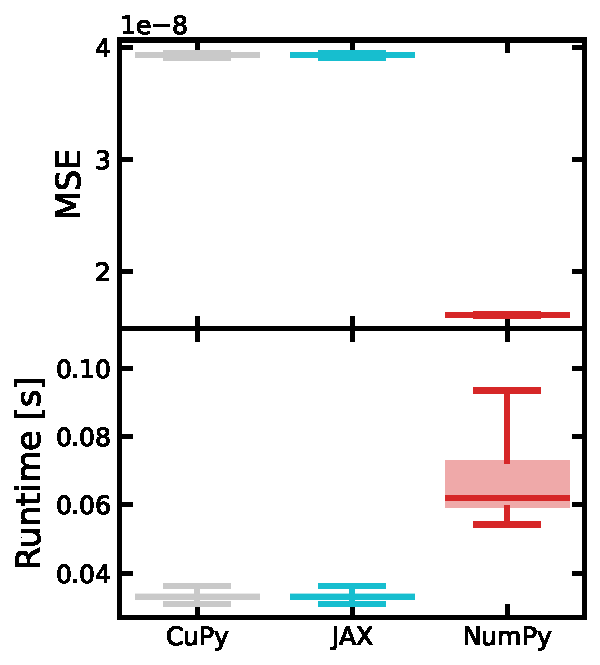
\includegraphics[width=1\linewidth]{figures/mse.pdf}
    \caption{Box plot of mean squared error (MSE) for forward‐then‐inverse WDM transforms on data with $N=2^{20}$, $N_f=2^{10}$, $N_t=2^{10}$. All three implementations (NumPy, JAX, CuPy) achieve MSE $< 10^{-8}$. The NumPy implementation has slightly lower MSE, while the JAX and CuPy implementations show MSE values that are marginally higher but still well below $10^{-8}$. Code to reproduce this plots can be found here:\url{pywavelet.github.io/pywavelet/examples/accuracy.html}.}
    \label{fig:mse_boxplot}
\end{figure}

All three implementations demonstrate a numerical accuracy of the transforms with a reconstruction MSE $<10^{-8}$. 
The NumPy backend yields the smallest reconstruction errors, likely because it does not have any GPU‐rounding differences. The JAX and CuPy versions incur slightly larger MSE, but still remain well below $10^{-8}$.
Moreover, as seen in the bottom panel of the figure, the JAX and CuPy implementations achieve substantial speedups despite this minor increase in MSE.

\subsection{Demonstration on Realistic Waveforms}
\label{subsec:demonstration_waveforms}

To illustrate the utility of \package\ on astrophysically relevant signals, we transform three different gravitational‐wave datasets into the WDM domain. Specifically, we transform (i) an \emph{extreme mass‐ratio inspiral} (EMRI) waveform, (ii) a set of \emph{verification galactic binaries} (VGB) and (iii) a \emph{massive black hole binary} (MBHB) signal. 
The VGB and MBHB data are obtained from the Radler LISA Data Challenge (via \url{https://lisa-ldc.lal.in2p3.fr/challenge1a}). 
The EMRI signal is generated using the \textsc{few} waveform, \textsc{Pn5AAKWaveform}~\cite{}, with the parameters YY.
Figure~\ref{fig:wdm_real_waveforms} displays both the frequency domain characteristic strain, and the WDM‐domain representations of these three signals. Each panel shows the time–frequency–WDM amplitude map obtained with the JAX implementation (on the GPU). The durations and transform runtimes for each dataset are listed in Table~\ref{tab:waveform_specs}.

\begin{figure*}[h]
    \centering
    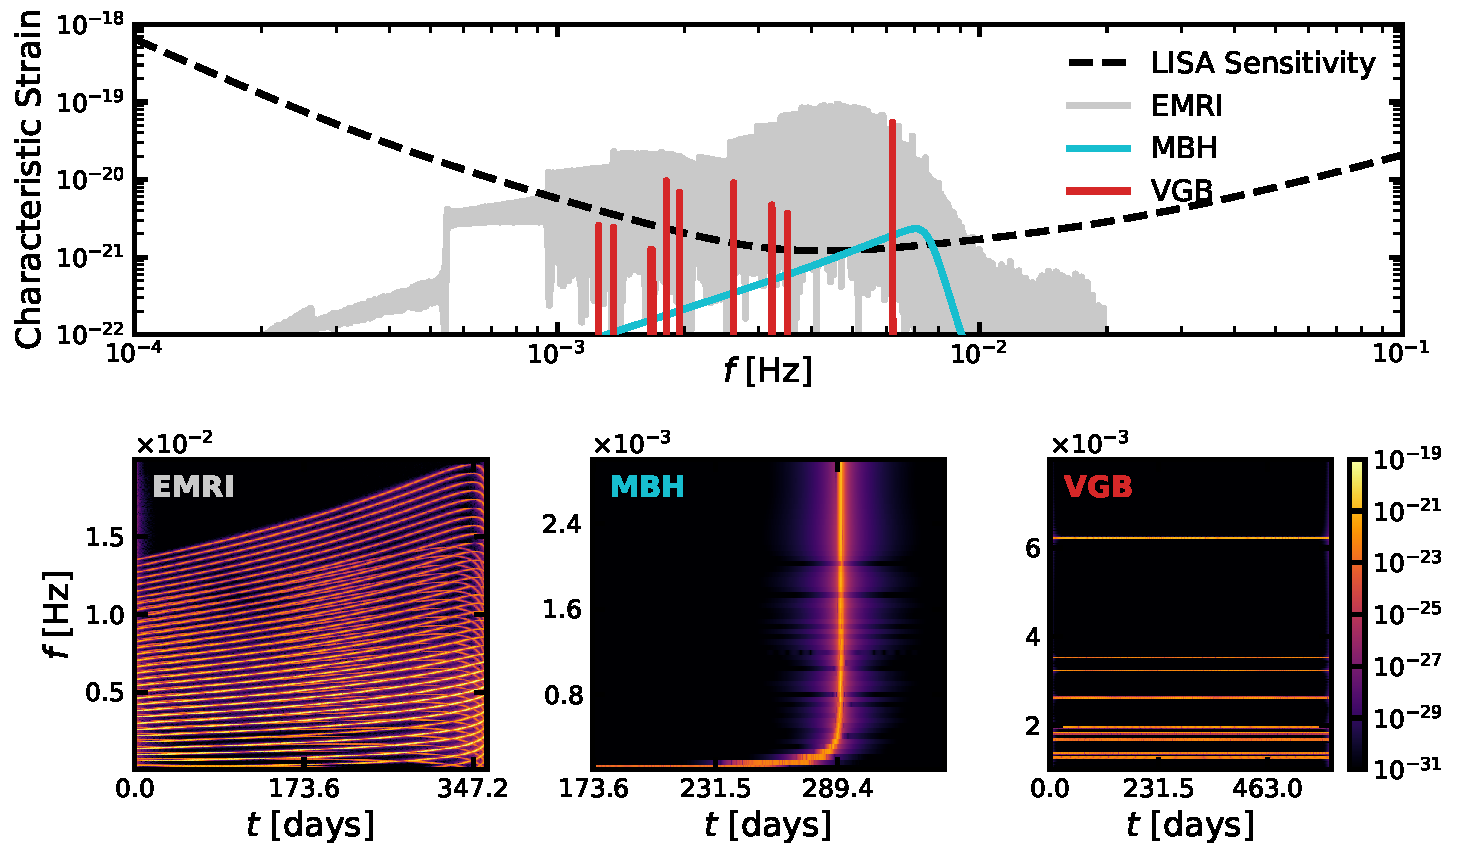
\includegraphics[width=1\linewidth]{figures/example_transforms.pdf}
    \caption{WDM‐domain representations of three astrophysical signals: (a) EMRI waveform; (b) verification binary ensemble; (c) massive black hole binary from the Radler LISA Data Challenge. All transforms computed with JAX on the GPU.}
    \label{fig:wdm_real_waveforms}
\end{figure*}

\begin{table*}[h]
    \centering
    \begin{tabular}{lccrrr}
        \toprule
        \textbf{Signal} & \textbf{Duration (s)} & \textbf{Data Length} & \textbf{NumPy Runtime (s)} & \textbf{JAX Runtime (s)} & \textbf{CuPy Runtime (s)} \\
        \midrule
        EMRI                   & $T_{\rm EMRI}$      & $N_{\rm EMRI}$     & $t_{\rm EMRI,\,\text{NumPy}}$ & $t_{\rm EMRI,\,\text{JAX}}$ & $t_{\rm EMRI,\,\text{CuPy}}$   \\
        Verification Binaries  & $T_{\rm VVB}$       & $N_{\rm VVB}$      & $t_{\rm VVB,\,\text{NumPy}}$  & $t_{\rm VVB,\,\text{JAX}}$  & $t_{\rm VVB,\,\text{CuPy}}$    \\
        MBH Binary (Radler)    & $T_{\rm MBHB}$      & $N_{\rm MBHB}$     & $t_{\rm MBHB,\,\text{NumPy}}$ & $t_{\rm MBHB,\,\text{JAX}}$ & $t_{\rm MBHB,\,\text{CuPy}}$   \\
        \bottomrule
    \end{tabular}
    \caption{Durations, data lengths, and runtimes for the WDM forward transform of three demonstration waveforms using NumPy (CPU), JAX (GPU), and CuPy (GPU).}
    \label{tab:waveform_specs}
\end{table*}

In Table~\ref{tab:waveform_specs}, $T_{\rm EMRI}$, $T_{\rm VVB}$, and $T_{\rm MBHB}$ denote the physical durations (in seconds) of the EMRI, verification binaries, and MBHB signals, respectively; $N_{\rm EMRI}$, $N_{\rm VVB}$, and $N_{\rm MBHB}$ are the corresponding number of time‐domain samples. 
The runtimes $t_{\rm EMRI,\,NumPy}$, $t_{\rm VVB,\,NumPy}$, and $t_{\rm MBHB,\,NumPy}$ were measured on the CPU using the NumPy backend. 
A corresponding GPU benchmark (JAX or CuPy) for each dataset is provided in the Appendix.

\subsection{Summary}
\label{subsec:summary}

The \package\ package enables both a straightforward NumPy‐based development path and high‐performance GPU‐accelerated execution via JAX and CuPy. 
For small data lengths ($N \lesssim 2^{20}$), the NumPy version is competitive or even faster due to its extremely low overhead. 
However, once $N$ exceeds $\sim 2^{20}$, the GPU‐accelerated versions achieve markedly lower runtimes while maintaining MSE well below $10^{-8}$. 
This combination of flexibility, accuracy, and performance makes \package\ a useful tool for time–frequency–WDM analysis of long-duration gravitational-wave signals.






\section{Applications of \package\ in Science (To be discussed, low priority!)}
\subsection{Basic section on gaps (Ollie + Avi)}
\begin{itemize}
\item Do some calculations to show what gaps do to WDM transform . 
\item Show correlated noise covariance matrix.
\item Show PE scheme with frequency domain vs time-frequency domain. Just use simple waveform. 
\end{itemize}

In order to deal with the gaps, it is sufficient to define the matrix $\mathbf{W_n}$ in such a way that
%
\begin{align}
\mathbf{W_n}=\begin{cases}
    \sqrt{2} \Delta t  \,\phi[j]\delta_{j+nN_f,k}&\qquad n\notin \text{gaps}\\
    0 &\qquad n\in \text{gaps}
\end{cases}
\end{align}
%
Since the matrix $\mathbf{W_n}$ is singular even in the untapped case, there is no further complication as the pseudo-inversion of $\mathbf{G}$ has to be done in the same way. In this case we find
%
\begin{align}
\mathbf{G}^\dagger&= \begin{pmatrix} \mathbf{W}_0\left(\bar{\mathbf{G}}^T\mathbf{G}\right)^{-1}\bar{\mathbf{F}}^T\\ \mathbf{W}_1\left(\bar{\mathbf{G}}^T\mathbf{G}\right)^{-1}\bar{\mathbf{F}}^T\\...\\ \mathbf{W}_{N_t-1}\left(\bar{\mathbf{G}}^T\mathbf{G}\right)^{-1}\bar{\mathbf{F}}^T
\end{pmatrix} \\ &=\begin{pmatrix} \mathbf{W}_0\\ \mathbf{W}_1\\...\\ \mathbf{W}_{N_t-1}
\end{pmatrix}\left(\bar{\mathbf{G}}^T\mathbf{G}\right)^{-1}\bar{\mathbf{F}}^T \\&\equiv\mathbf{W}\left(\bar{\mathbf{G}}^T\mathbf{G}\right)^{-1}\bar{\mathbf{F}}^T
\end{align}
%

\subsection{Chirping sinusoid, consequences for GB searches (Quentin, Giorgio, Lorenzo)}
\begin{itemize}
\item Timing comparisons between pywavelet and direct generation freq in domain. We could use \texttt{fastGB} and then transform. 
\item Parameter estimation simulation comparing WDM and frequency domain. Overlapping posteriors. Could do this with an EMRI source or MBH source. This wouldn't be hard. 
\end{itemize}
\section{Conclusions (all)}
\begin{itemize}
\item Summarise paper quickly. Discuss advantageous and disadvantageous. 
\item Speak about speed of transform code. It may not always be possible to generate signals directly in WDM domain? 
\item Discussion about including our code within LISA framework?
\end{itemize}




\section*{Data and Software Availability}
The software developed for this research is available on GitHub under the MIT License~\citep{}.
Documentation and examples of the software can be found at \url{url}. 
The data products for this work have been archived on Zenodo~\cite{X}.





\begin{acknowledgments}
We thank XYZ
GM acknowledges support from the Imperial College London Schr\"odinger Scholarship scheme.
\end{acknowledgments}


\vspace{4mm}
\noindent\textit{Software used:}
\newcommand{\python}{~\cite{python2020}}
\newcommand{\tensorflowProb}{~\cite{tensorflow, tensorflowProb}}
\newcommand{\numpy}{~\cite{numpy}}
\newcommand{\scipy}{~\cite{scipy}}
\newcommand{\pandas}{~\cite{pandas}}
\newcommand{\matplotlib}{~\cite{matplotlib}}
\newcommand{\jupyterbook}{~\cite{jupyterbook}}


% \section{GW Data analysis}\label{sec:data_an}


% We define the useful quantities which are useful to perform GW data analysis and the parameter estimation in perfect analogy to what has already been done in the frequency domain. In particular, we refer to \cite{Veitch:2009hd} if the reader is interested to a precise comparison.
% The data stream will be
% %
% \begin{align}
% d_{nm}=h_{nm}+n_{nm}
% \end{align}
% %
% where $d_{nm}$ is the datastream in the wavelet domain, $h_{nm}(\theta)$ the GW signal and $n_{nm}$ the noise.
% For a template search, we need to match filter the observed datastream with some functions $Q_{nm}(\theta)$ of some theoretical parameters $\theta$, that (as we will show) depend on our bank of waveform templates in the wavelet domain
% %
% \begin{align}
% d_f\equiv \sum_n\sum_m d_{nm}Q_{nm}(\theta)
% \end{align}
% %
% The expected value and the variance of our filtered datastream $d^f$ will be (a noise dominated datastream is assumed)
% %
% \begin{align}
% \langle d_f \rangle&= \sum_{nm} h_{nm}Q_{nm}(\theta)\nonumber\\
% \langle |d_f|^2 \rangle&=\sum_{nm} |Q_{nm}(\theta)|^2S_{nm}
% \end{align}
% %
% where $S_{nm}$ is the noise power spectral density in the wavelet domain. \textcolor{blue}{[Giorgio: yet to understand all the dimensions and factors 2 to define $S_{nm}$ eheh]}.
% The Signal-to-Noise Ratio (SNR) squared in this case will be
% %
% \begin{align}
% \rho=\frac{\left|\sum_{nm} h_{nm}Q_{nm}(\theta)\right|^2}{\sum_{nm} |Q_{nm}(\theta)|^2S_{nm}}
% \end{align}
% %
% The interpretation of this formula is analogous to what happens in the frequency domain, where it can be seen as a scalar product in the vector space of the functions in the wavelet domain. If we define a scalar product between two generic wavelet functions $a_{nm}$ and $b_{nm}$ as
% %
% \begin{align}
% \left(a|b\right)\equiv \sum_{nm} a^*_{nm} b_{nm} S_{nm}
% \end{align}
% %
% then it is easy now to see that the choice for the filter that maximises the SNR above is $Q_{nm}(\theta)=\frac{h^*_{nm}}{S_{nm}}$, which leads to the optimally-filtered value for the SNR$^2$
% %
% \begin{align}
% \rho_{\rm opt}=\sum_{nm}\frac{|h_{nm}|^2}{S_{nm}}
% \end{align}
% %


% \subsection{Likelihood function and Fisher matrix}

% The Likelihood function of the data, given some choice of the theoretical parameters $\theta$ can be built in a similar way to what we do for the SNR, under the assumption of a noise dominated signal, in the same way of \cite{Cornish:2020odn}
% %
% \begin{align}\label{eq:likelihood_def}
% \log\mathcal{L}(d|\theta) &=-\frac{1}{2}\left( \sum_{n m} {\rm ln}(2\pi S_{nm})+\chi^2(\theta)\right) \nonumber\\
% \chi^2(\theta)&=\sum_{n m}\frac{|d_{nm} -h_{nm}(\theta)|^2}{S_{nm}} 
% \end{align}
% %
% \textcolor{blue}{[Giorgio: In Cornish the numerator does not have a $||^2$ but a $()^2$. I think the wavelet coefficients in general are complex, so we should write as I did: is that right?]}
% where we are exploiting the diagonality of the noise covariance matrix in the wavelet domain.
% The Fisher Matrix is built from the second derivatives of the chi-squared on the theoretical parameters $\theta$, evaluated at the fiducial value $\hat\theta$, which corresponds to the maximum of the distribution, such that $d_{nm}=h_{nm}(\hat\theta)$.
% %
% \begin{align}
% \mathcal{F}_{\theta\theta'}\equiv\frac{1}{2}\frac{\partial^2\chi^2}{\partial\theta\partial\theta'}_{\big| \substack{\theta=\hat\theta \\ \theta'=\hat\theta'}}=\sum_{nm}\frac{1}{S_{nm}}\left(\frac{\partial h_{nm}(\theta)}{\partial\theta}_{\big|_{\theta=\hat\theta}}\frac{\partial h_{nm}(\theta')}{\partial\theta'}_{\big|_{\theta'=\hat\theta'}}\right)
% \end{align}
% %
% where the last equality follows from the explicit writing of \eqref{eq:likelihood_def}. We obtain therefore the approximation for the chi-squared\footnote{See \cite{Dodelson} for more details on the derivation of the Fisher matrix}.
% %
% \begin{align}
% \chi^2_F\equiv \left(\theta-\hat\theta\right)^T\mathcal{F}_{\theta\theta'}\left(\theta'-\hat\theta'\right)
% \end{align}



% \section{Applications}

% \subsection{Gaps}


% \subsection{Monochromatic signal}


% \subsection{Galactic binary (chirping) signal}

% \textcolor{blue}{[Giorgio: I moved what was here to the newborn section \textit{Galactic binary signal} in the big overleaf file]}

\appendix




%------

\section{Inverse-forward-inverse wavelet transform (Giorgio)}
I decompose my signal in the WDM domain
%
\begin{align}
\tilde x_l=\sum_{n=0}^{N_t-1}\sum_{m=0}^{N_f}\tilde g_{nm}[l] w_{nm}
\end{align}
%
where $N=N_fN_t$
%
\begin{align}
\tilde x_l=\sum_{k=0}^{N-1} e^{2\pi i k l/N}x_k
\end{align}
%
The basis elements are defined (Farr) as
%
\begin{align}
\tilde{g}_{n m}(f):= \begin{cases}
e^{-4\pi i n f \Delta T} \tilde{\varphi}(f), & m=0 \\
\frac{1}{\sqrt{2}}e^{-2 \pi i n f \Delta T}\left(C_{n m} \tilde{\varphi}(f-m \Delta F)+C_{n m}^* \tilde{\varphi}(f+m \Delta F)\right), & 0<m<N_f \\
e^{-4 \pi i n f \Delta T}\left(\tilde{\varphi}(f-m \Delta F)+\tilde{\varphi}(f+m \Delta F)\right), & m=N_f
\end{cases}
\end{align}
%
for $m=0,...,N_f$ and $n=0,...,N_t-1$. We first verify the (quasi)orthonormality condition with
%
\begin{align}
\sum_l \tilde{g}_{n 0}(l)\tilde{g}^*_{n' 0}(l)&=\sum_l e^{-4\pi i (n-n') l/N_t} \tilde{\varphi}(f[l])\tilde{\varphi}(f[l])\simeq\delta_{nn'}\nonumber\\
\sum_l \tilde{g}_{n m}(l)\tilde{g}^*_{n' 0}(l)&=\frac{1}{\sqrt{2}}\sum_l e^{-2\pi i (n-n') l/N_t} \left(C_{n m} \tilde{\varphi}(f-m \Delta F)+C_{n m}^* \tilde{\varphi}(f+m \Delta F)\right)\tilde{\varphi}(f[l])\simeq\nonumber\\
&\simeq\frac{\delta_{nn'}}{\sqrt{2}}\sum_l  \left(C_{n m} \tilde{\varphi}(f-m \Delta F)+C_{n m}^* \tilde{\varphi}(f+m \Delta F)\right)\tilde{\varphi}(f[l])\simeq 0\nonumber\\
\sum_l \tilde{g}_{n m}(l)\tilde{g}^*_{n' m'}(l)&=\frac{1}{2}\sum_l e^{-2\pi i (n-n') l/N_t} \left(C_{n m} \tilde{\varphi}(f-m \Delta F)+C_{n m}^* \tilde{\varphi}(f+m \Delta F)\right)\times \nonumber\\
&\left(C_{n' m'}^* \tilde{\varphi}(f-m' \Delta F)+C_{n' m'} \tilde{\varphi}(f+m' \Delta F)\right)\simeq\nonumber\\
&=\frac{\delta_{nn'}\delta_{mm'}}{2}\sum_l \left(C_{n m}C_{n m}^* \tilde{\varphi}^2(f-m \Delta F)+C_{n m}^*C_{n m} \tilde{\varphi}^2(f+m \Delta F)\right)=\nonumber\\
&=\delta_{nn'}\delta_{mm'}C_{n m}C_{n m}^*=\delta_{nn'}\delta_{mm'}
\end{align}
%
We therefore can write the forward transform
%
\begin{align}
w_{nm}=\sum_{l=0}^{N-1} \tilde{x}_l \tilde g_{nm}^*(f[l])
\end{align}
%
Then we have to note that in order to discretize the equation we must impose
%
\begin{align}
f[l]=\begin{cases}
    l & 0\leq l< N/2 \\
    l-N & N/2\leq l<N
\end{cases}\times df
\end{align}
%

\subsection{The general case: $m>0$}
Putting all together, for $m>0$ we find
%
\begin{align}
w_{nm}&=\frac{1}{\sqrt{2}}\sum_{l=0}^{N/2-1} \tilde{x}_l e^{2\pi iln/N_t}\left[C_{nm}^*\tilde{\varphi}\left((l-\frac{mN_t}{2})df\right)+C_{nm}\tilde{\varphi}\left((l+\frac{mN_t}{2})df\right)\right]+\nonumber\\
&+\frac{1}{\sqrt{2}}\sum_{l=N/2+1}^{N-1} \tilde{x}_l e^{2\pi i(l-N)n/N_t}\left[C_{nm}^*\tilde{\varphi}\left((l-N-\frac{mN_t}{2})df\right)+C_{nm}\tilde{\varphi}\left((l-N+\frac{mN_t}{2})df\right)\right]
\end{align}
%
Now, one can do the change of variables $l\to N-l$ in the second term and notice that $\tilde{x}_{N-l}=\tilde{x}^*_l$, and that $\tilde{\varphi}(-f)=\tilde{\varphi}(f)$. After some straightforward algebra, one realizes that the second term is exactly the complex conjugate of the first. Therefore we can write
%
\begin{align}\label{wnm_m_general}
w_{nm}&=\sqrt{2}\,\Re\left[\sum_{l=1}^{N/2-1} \tilde{x}_l e^{2\pi iln/N_t}\left[C_{nm}^*\tilde{\varphi}\left((l-\frac{mN_t}{2})df\right)+C_{nm}\tilde{\varphi}\left((l+\frac{mN_t}{2})df\right)\right]\right]+\nonumber\\
&+ \frac{1}{\sqrt{2}}\tilde{x}_0 \left[C_{nm}^*\tilde{\varphi}\left(-\frac{mN_t}{2}df\right)+C_{nm}\tilde{\varphi}\left(\frac{mN_t}{2}df\right)\right]\nonumber\\
&+ \frac{1}{\sqrt{2}}\tilde{x}_{N/2}e^{\pi i n N_f} \left[C_{nm}^*\tilde{\varphi}\left((\frac{N}{2}-\frac{mN_t}{2})df\right)+C_{nm}\tilde{\varphi}\left((\frac{N}{2}+\frac{mN_t}{2})df\right)\right]\nonumber\\
&=\sqrt{2}\,\Re\sum_{l=1}^{N/2-1} \tilde{x}_l e^{2\pi iln/N_t}C_{nm}^*\tilde{\varphi}\left((l-\frac{mN_t}{2})df\right)\nonumber\\
&=\sqrt{2}(-1)^{nm}\,\Re\sum_{l'=-N_t/2}^{N_t/2} \tilde{x}_{l'+\frac{mN_t}{2}} e^{2\pi il'n/N_t}C_{nm}^*\tilde{\varphi}(l\,df)
\end{align}
%
where the second equality holds since $\tilde{\varphi}(l\,df)$ is non zero only for $-N_t/2\leq l\leq N_t/2$ and the last one follows from the substitution $l'= l-\frac{mN_t}{2}$. Please note that this equation is, up to a normalization, eq.17 by Cornish.

\subsection{The DC frequency $m=0$}
In this case
%
\begin{align}
w_{n0}&=\sum_{l=0}^{N/2-1} \tilde{x}_l e^{4\pi iln/N_t}\tilde{\varphi}(l\,df)
+\sum_{l=N/2}^{N-1} \tilde{x}_l e^{4\pi i(l-N)n/N_t}\tilde{\varphi}((l-N)\,df)
\nonumber\\
&=2\,\Re\left[\sum_{l=1}^{N_t/2} \tilde{x}_{l} e^{4\pi iln/N_t}\tilde{\varphi}(l\,df)\right]+\tilde{x}_0\tilde{\varphi}(0)
\end{align}
%

\subsection{Inverse}
Let's compute
%
\begin{align}
\tilde x_l &= \sum_n\sum_m g_{nm}(l) w_{nm}=\sum_n g_{n0}(l) w_{n0}+\sum_n \sum_{m\neq 0} g_{nm}(l) w_{nm}=\nonumber\\
&=\sum_n e^{-2\pi iln/N_t}\tilde{\varphi}(f(l))\left(\sum_{l'=1}^{N_t/2} (\tilde{x}_{l'} e^{2\pi il'n/N_t}\tilde{\varphi}(l'\,df)+\tilde{x}^*_{l'} e^{-2\pi il'n/N_t}\tilde{\varphi}(l'\,df))+\tilde{x}_0\tilde{\varphi}(0)\right)+\nonumber\\
&+\frac{1}{\sqrt{2}}\sum_n\sum_m e^{-2\pi iln/N_t}\left[C_{nm}\tilde{\varphi}\left(f(l)-\frac{mN_t}{2}df\right)+C_{nm}^*\tilde{\varphi}\left(f(l)+\frac{mN_t}{2}df\right)\right]\times\nonumber\\
&\times\sqrt{2}\sum_{l'=1}^{N/2-1}\left[e^{-2\pi il'n/N_t}\tilde x^*_{l'}C_{nm}\tilde{\varphi}\left((l'+\frac{mN_t}{2})df\right)+e^{2\pi il'n/N_t}\tilde x_{l'}C_{nm}^*\tilde{\varphi}\left((l'-\frac{mN_t}{2})df\right)\right]=\nonumber\\
&=
N_t\tilde x_l\tilde{\varphi}^2(l\,df)\theta\left(\frac{N_t}{2}-l\right)+N_t\tilde x_l\tilde{\varphi}^2((l-N)\,df)\theta\left(l-N+\frac{N_t}{2}\right)+N_t\sum_m \theta\left(l-\frac{(m+1)N_t}{2}\right)\theta\left(\frac{(m-1)N_t}{2}-l\right)\tilde\varphi^2(l\,df)\tilde x_l=\nonumber\\
&=\tilde x_l
\end{align}
%
where the last equality holds since $\tilde\varphi(l\,df)\simeq \frac{1}{\sqrt{N_t}}$

\section{Normalization of the Meyer window}\label{app:normalization_Meyer}

We recall the definition of the Meyer window functions in the frequency domain $\tilde{\phi}(\omega)$ in eq. \eqref{eq:meyer_window_freq}
\begin{align}
\tilde\phi(\omega)=\left\{\begin{array}{lr}
\frac{1}{\sqrt{\Delta \Omega}} & |\omega|<A \\
\frac{1}{\sqrt{\Delta \Omega}} \cos \left[\frac{\pi}{2}\,\nu_d\left( \frac{|\omega|-A}{B}\right)\right] &A \leq|\omega| \leq A+B
\end{array}\right.\;,
\end{align}
with
\begin{align}
\nu_d(x)=\frac{\int_0^x y^{d-1}(1-y)^{d-1} d y}{\int_0^1 y^{d-1}(1-y)^{d-1} d y}\;.
\end{align}
%
We compute, defining $a=\frac{A}{\Delta\Omega}$ and remembering that $B=\Delta\Omega-2A$
%
\begin{align}
&\int_{-\infty}^{+\infty} d\omega\, \tilde{\phi}^2(\omega)=2\int_{0}^{A} d\omega\, \frac{1}{\Delta\Omega}+2\int_{A}^{A+B} d\omega\, \frac{1}{\Delta\Omega}\cos^2 \left[\frac{\pi}{2}\,\nu_d\left( \frac{\omega-A}{\Delta\Omega-2A}\right)\right]=\nonumber\\
&=2a+2\int_a^{1-a}dx\,\cos^2 \left[\frac{\pi}{2}\,\nu_d\left( \frac{x-a}{1-2a}\right)\right]=2a+2\int_0^{1-2a}dy\,\cos^2 \left[\frac{\pi}{2}\,\nu_d\left( \frac{y}{1-2a}\right)\right]=\nonumber\\
&=2a+2(1-2a)\int_0^1 dz\,\cos^2 \left[\frac{\pi}{2}\,\nu_d\left( z\right)\right]=2a+(1-2a)\int_0^1 dz\, +(1-2a)\int_0^1 dz\,\cos \left[\pi\,\nu_d\left( z\right)\right]=\nonumber\\
&=1
\end{align}
%
since the last term is equal to 0:
%
\begin{align}
\int_0^1 dz\,\cos \left[\pi\,\nu_d\left( z\right)\right]=\int_0^1 dz\,\cos \left[\pi\,\nu_d\left( 1-z\right)\right]=\int_0^1 dz\,\cos \left[\pi\,(1-\nu_d\left( z\right))\right]=-\int_0^1 dz\,\cos \left[\pi\,\nu_d\left( z\right)\right]
\end{align}

%-----

\bibliographystyle{plain} % We choose the "plain" reference style
\bibliography{bib} % Entries are in the refs.bib file

\end{document}